\section{Protocollo di scambio}
Il protocollo utilizzato per lo scambio di messaggi è molto semplice e si basa sulla ricezione da parte del server di comandi e del successivo invio di esito dell'operazione al client. Ogni operazione, infatti, può portare all'invio da parte del server di una risposta \textbf{success} o \textbf{failure} \footnote{Si è scelto di generalizzare quanto più possibile il concetto di \textit{messaggio}, così da includervi anche quelli di risposta}.

Dunque, tutti i tipi di messaggi scambiati sono inglobati all'interno dell'enum \textbf{Commands}:
\begin{multicols}{2}
	\begin{itemize}
		\item LOGIN
		\item LOGOUT
		\item CREATE
		\item EDIT
		\item EDIT\_END
		\item SHOW\_SECTION
		\item SHOW\_DOCUMENT
	\end{itemize}
	\begin{itemize}
		\item LIST
		\item SHARE
		\item SUCCESS
		\item FAILURE
		\item NEW\_NOTIFICATIONS
		\item EXIT
	\end{itemize}
\end{multicols}
Per ognuno di questi, viene definito un array di tipi, così da dare la possibilità al client di controllare che il tipo di dato degli argomenti inviati sia corretto e per permettere al server di inferire l'ordine ed il tipo di \textit{receive()} da effettuare per ricostruire i dati inviati. Nella sezione \ref{rappresentazione_dei_dati} verrà chiarito meglio in che modo questi vengano scambiati a partire dai loro tipi.

Il protocollo prevede anche delle procedure per lo scambio di stream di dati, utili per l'invio e ricezione da parte del server del contenuto dei file rappresentanti le sezioni dei documenti o la loro concatenazione\footnote{Infatti, durante l'esecuzione del comando \textbf{SHOW\_DOCUMENT}, il server si serve della concatenazione di più stream di file per crearne uno unico da poter inviare al client, sfruttando la funzione appena descritta} .
L'invio di stream dev'essere \underline{necessariamente} preceduto da un normale invio di esito da parte del server per evitare la rottura del protocollo.

\paragraph{Approccio Funzionale}
L'approccio utilizzato nella stesura del codice relativo all'implementazione del protocollo è fortemente funzionale e segue le tecniche più moderne, coinvolgendo la definizione di appositi handler chiamati in base all'esito delle operazioni. Il listing \ref{lst:functional} è un chiaro esempio di come la programmazione funzionale venga impiegata nell'utilizzo del protocollo.

\begin{lstlisting}[language=java, caption="Frammento in cui si evidenzia l'approccio funzionale del protocollo", label={lst:functional}, float]
private void documentsList() {
	if (session != null)
		Communication.send(
			clientOutputStream,
			clientInputStream,
			System.out::println, System.err::println,
			Commands.LIST);
	else System.err.println("You're not logged in");
}
\end{lstlisting}

\subsection{Rappresentazione dei dati}\label{rappresentazione_dei_dati}
Vengono utilizzati degli oggetti di tipo \textbf{DataInputStream} e \textbf{DataOutputStream} rispettivamente per la ricezione e l'invio dei dati sul socket, per riuscire ad inviarne la corretta rappresentazione in byte\footnote{Molto utile per l'invio corretto di interi, per esempio, evitando di dover effettuare interpretazione di testo contenente la loro rappresentazione}. Se per gli interi questo approccio risulta sufficiente ad assicurarne correttamente lo scambio, per le stringhe si è dovuto far affidamento all'invio di una informazione addizionale: il numero di byte che le compongono. Infatti, ogni volta che si presenta la necessità di inviare una stringa, si procede prima alla \textit{send()} del numero di byte che la compongono e successivamente a quella dell'array dei dati. In questo modo, utilizzando l'approccio contrario, è possibile sapere di preciso quanti byte appartenenti alla stringa da ricevere prelevare dal buffer.

\begin{figure}[h]
	\caption{Schema di rappresentazione delle stringhe}
	\centering
	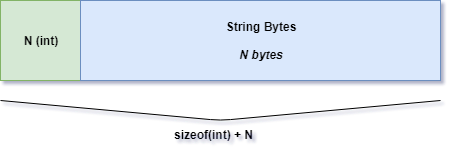
\includegraphics[scale=0.6]{assets/string_representation.png}
\end{figure}

\subsection{Sistema di notifiche}
Il sistema di notifiche è un esempio 